% 第40回情報理論とその応用シンポジウム予稿集 
% 日本語原稿

\documentclass{jarticle}
\usepackage{sita2017,amsmath,amssymb,amsfonts}
\usepackage[dvipdfmx]{graphicx}
\title{
  近似的メッセージ伝播法に基づくパイロット汚染の軽減 \\
  Reduction of pilot contamination based on approximate message propagation method
}
%
\author{
藤塚 拓実
  \thanks{ 
    〒441-8580 愛知県豊橋市天伯町雲雀ヶ丘1-1 豊橋技術科学大学 電気・電子情報工学専攻 通信信号処理研究室 Communication \& Signal Processing Lab., Department of Electrical and Electronic Information Engineering, Toyohashi University of Technology
E-mail: {\tt fujitsuka@\allowbreak
comm.\allowbreak
ee.\allowbreak
tut.\allowbreak
ac.\allowbreak
jp}
  }\\
  Fujitsuka Takumi
%
%   \and
% %第二著者名(和文)
%   \thanks {
% %第二著者の所属と住所(和文と英文)
% %もし第一著者と同じならば,\thanks{}の代りに\samethanks{1}を使ってください.
%   }\\
% %第二著者名(英文)
%
}
\abstract{
%英文のアブストラクト
2020年を目標として第5世代無線通信(5G)の標準化が推進されている.5Gにおける最も重要な技術として大規模MIMO(Massive MIMO)がある.大規模MIMOではダウンリンクにおいて,ビームフォーミングを行うことで端末ごとの通信を最適化するが,そのためには通信路状態情報(CSI)を得る必要がある.CSIを得るためには,アップリンクにおいてユーザがパイロット信号と呼ばれる既知信号を基地局に送信することでCSIを推定する.その際,基地局間干渉であるパイロット汚染と呼ばれる現象が発生する.本研究では,アップリンクにおける大規模MIMOのシステムにおいて,パイロット汚染を軽減するため,パイロットの送信タイミングを基地局ごとに時間シフトさせた上で,近似的メッセージ伝播法(AMP)を使用して,CSIとデータを同時に推定することを目標とする.昨年度までの研究ではAMPの収束性に難があったが,アルゴリズムの初期の変更とダンピングを駆使することで収束性の向上を果たした.また,基地局ごとの電力差とデータにスパース性を持たせた場合の検証を試みた.
}
% \keywords{
% %英語のキーワード(3 - 5語)
% }
  
\begin{document}
\maketitle

\section{はじめに}
移動通信の標準化団体3GPPや総務省,企業,大学などが連携し,国内外で2020年を目標として第5世代無線通信(5G)の標準化が推進されている\cite{5gmf}.5Gにおける最も重要な技術として大規模MIMO(Massive MIMO)\cite{Marzetta}がある.大規模MIMOではダウンリンクにおいて,ビームフォーミングを行うことで端末ごとの通信を最適化するが,そのためには通信路状態情報(Channel State information : CSI)を得る必要がある.CSIを得るためには,アップリンクにおいてユーザがパイロット信号と呼ばれる既知信号を基地局に送信することでCSIを推定する.しかし,コヒーレンス時間によってパイロット信号の長さが制限されるため,隣接する基地局と同一のパイロット信号を使用することになり,同一のパイロット信号することでCSIの推定を困難にする現象をパイロット汚染\cite{Marzetta}と呼ぶ.

パイロット汚染を軽減する方法として,基地局ごとにパイロットの送信タイミングを時間シフトさせて送信する手法が提案されている\cite{Appaiah}.本研究では,パイロット信号を基地局で時間シフトさせ,復号アルゴリズムとして樺島が定式化した近似的メッセージ伝播法(Approximate Message Passing :AMP)\cite{kabashima}を使用し,数値シミュレーションによってアルゴリズムの有用性を検証する.
\section{想定するシステム}
複数ユーザが基地局に情報を送るアップリンクを想定し,ユーザ数を$K$,受信アンテナ数を$N$とし,ユーザは単一の送信アンテナを持つことを想定する.また,簡単のため,フェージング係数が観測時間$T$の間一定であるブロックフェージング通信路を仮定する.受信信号$\boldsymbol{Y} \in \mathbb{C}^{N \times T}$は(\ref{eq:sys})式にて与えられる.
\begin{equation}
    \label{eq:sys}
    \boldsymbol{Y} = \frac{1}{\sqrt{N}}\boldsymbol{HX+W}.
\end{equation}
$1/\sqrt{N}$は正規化定数であり,アンテナ数の上昇による電力の上昇を抑える.$\boldsymbol{X}\in\mathbb{C}^{K\times T}$は全ユーザの送信信号であり,$\boldsymbol{H}\in\mathbb{C}^{N\times K}$はすべてのユーザとアンテナ間のフェージング係数でありCSIに相当する.ここで,$\boldsymbol{H}$に関して,すべての行列成分は,互いに独立で同一の分布(independent and identically distribution : i.i.d)のレイリーフェージングに従うと仮定する.具体的には,それぞれが独立した円対称複素ガウス雑音(Circularly Symmetric Complex Gaussian : CSCG)であり,分散は1とした.また,$\boldsymbol{W}\in\mathbb{C}^{N\times T}$は受信時に生じる雑音のことであり,それぞれが独立した円対称複素ガウス雑音で,分散は定数$N_0$とした.

基地局が2つ隣接していると仮定し(図\ref{fig:system}参照),$\boldsymbol{X}$の上半分$K/2$が自身の基地局のユーザ,下半分$K/2$ユーザが隣接セルのユーザとし,パイロット信号$\boldsymbol{P}$を時間シフトさせて配置させるため,$\boldsymbol{X}$は(\ref{eq:SendSignal})式で表される.$\boldsymbol{P}$以外の$\boldsymbol{X}$はすべて基地局には未知のデータである.
\begin{equation} 
	\label{eq:SendSignal}
	\boldsymbol{X} =  \left(
		\begin{array}{cccc}
			\boldsymbol{X}_{11} &\boldsymbol{X}_{12} &\boldsymbol{P}\\
			\boldsymbol{P} &\boldsymbol{X}_{21} &\boldsymbol{X}_{22}
		\end{array}
	\right).
\end{equation}
\begin{figure}[htbp]
    \begin{center}
     \includegraphics[width=80mm]{./system.png}
    \end{center}
    \caption{想定するシステム}
    \label{fig:system}
\end{figure}
\section{近似的メッセージ伝播法 AMP}
近似的メッセージ伝播法は,人口知能分野で提案された確率伝播法(Belief Propagation BP)を基礎として発展した統計学的手法であり.もともとは,圧縮センシングの分野で提案された手法である[9].樺島の手法を今回のシステムに適応すると,通信路(CSI)$\boldsymbol{H}$を推定する.データ推定に分けることができ,お互いの推定結果を使って推定を繰り返すことで解を得るアルゴリズムとなる.このとき計算する値はそれぞれの平均と分散である.
\section{結果}
樺島AMPアルゴリムの収束性にまだまだ問題があり,前年度までの研究では,パイロット信号$Tp$がユーザ数$K$の倍以上存在しなければ解が発散し,また推定値が振動する問題が発生した.

本年度では,分散の初期値を変更し,ダンピング\cite{vila}によって$Tp=K$でも解を収束することができた.具体的には,初回の通信路推定にて,データ推定の分散を0で初期化し,ダンピング係数を$0.5$にすることで解を収束させた.

さらに,基地局間の距離を考慮し,各ユーザに電力の差異を考慮した場合のシミュレーションを行った.基地局間電力差を2倍にして数値シミュレーションを行った結果,はじめの反復の時は電力差がある場合の結果が通信路推定,BERともに優れていたが,最終的な結果としては反復を繰り返すと,基地局間電力差がない結果と比較してがBERでは$40\%$通信路推定のMSEでは$18\%$悪化している.

また,データのスパース性を高めて推定値の向上を図った.結果として,データの伝送
レートを0.1にしたところ,BERでは$99\%$向上し,通信路推定のMSEでは$87\%$悪化していた.つまり,データ推定の精度は向上するが,通信路推定が犠牲になる.

なお,上記の結果のシミュレーション条件はアンテナ数$N=128$,ユーザ数$K=32$,観測時間$T=128$,パイロット長$Tp=32$であり,反復回数は通信路推定,データ推定をそれぞれ10回ずつ反復し,この二つの推定を合計10回行っている.BERの比較を図\ref{fig:result}に示す.

初回の反復にて分散の初期値を0にすることで推定値が向上する理由として,データ推定を行っていない状態では,未知のデータが通信路推定を妨げるため,分散を0にすることでパイロット信号のみで通信路を推定を行うことで解が収束したと考えられる.また,初回のデータ推定では,パイロット信号を非同期にすることで干渉をうまく計算できないため,通信路の分散を0にすることで解が改善した.また,電力差が生じたときに最終的な結果が悪くなる理由としては,電力差がない場合に比べて,データの電力が小さくなり,通信路推定の結果が低下するため最終的な結果が悪くなる.しかし,電力差が完全に無い場合と比較するにはまだ検討の余地がある.スパース性を高めた場合も同様に,BERの面では利点があるように見受けられるが,送信レートは低くなっているため,比較にはまだ検討が必要である.

\begin{figure}[htbp]
    \begin{center}
     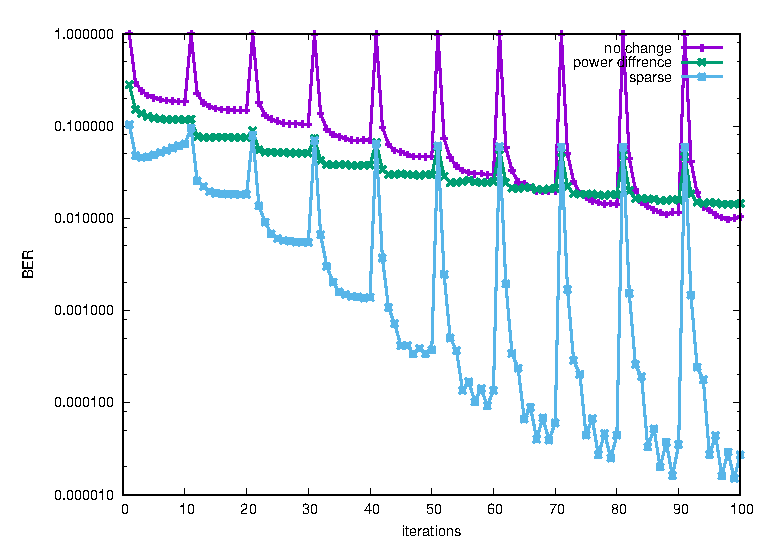
\includegraphics[width=80mm]{./result.eps}
    \end{center}
    \caption{BERの比較}
    \label{fig:result}
\end{figure}
\bibliographystyle{ieeetr}
\bibliography{reference}
\end{document}

% end of file
